%===============================================================================
% LaTeX sjabloon voor de graduaatsproef Programmeren aan HOGENT
% Meer info op https://github.com/HoGentPRG/latex-hogent-report
%===============================================================================

\documentclass[dutch,dit,thesis]{hogentreport}

% TODO:
% - If necessary, replace the option `dit`' with your own department!
%   Valid entries are dbo, dbt, dgz, dit, dlo, dog, dsa, soa
% - If you write your thesis in English (remark: only possible after getting
%   explicit approval!), remove the option "dutch," or replace with "english".

\usepackage{lipsum} % For blind text, can be removed after adding actual content

%% Pictures to include in the text can be put in the graphics/ folder
\graphicspath{{../graphics/}}

%% For source code highlighting, requires pygments to be installed
%% Compile with the -shell-escape flag!
%% \usepackage[chapter]{minted}
%% If you compile with the make_thesis.{bat,sh} script, use the following
%% import instead:
\usepackage[chapter,outputdir=../output]{minted}
\usemintedstyle{solarized-light}

%% Formatting for minted environments.
\setminted{%
    autogobble,
    frame=lines,
    breaklines,
    linenos,
    tabsize=4
}

%% Ensure the list of listings is in the table of contents
\renewcommand\listoflistingscaption{%
    \IfLanguageName{dutch}{Lijst van codefragmenten}{List of listings}
}
\renewcommand\listingscaption{%
    \IfLanguageName{dutch}{Codefragment}{Listing}
}
\renewcommand*\listoflistings{%
    \cleardoublepage\phantomsection\addcontentsline{toc}{chapter}{\listoflistingscaption}%
    \listof{listing}{\listoflistingscaption}%
}

% Other packages not already included can be imported here

%%---------- Document metadata -------------------------------------------------
% TODO: Replace this with your own information
\author{Thomas Gielen}
\supervisor{Dhr. F. Van Houte}
\cosupervisor{Mevr. S. Beeckman}
\title%
    {Back-end: Spring Boot}
\academicyear{\advance\year by -1 \the\year--\advance\year by 1 \the\year}
\examperiod{1}
\degreesought{\IfLanguageName{dutch}{Graduaat in het Programmeren}{Associate of applied computer science}}
\partialthesis{false} %% To display 'in partial fulfilment'
%\institution{Internshipcompany BVBA.}

%% Add global exceptions to the hyphenation here
\hyphenation{back-slash}

%% The bibliography (style and settings are  found in hogentthesis.cls)
\addbibresource{bachproef.bib}            %% Bibliography file
\addbibresource{../voorstel/voorstel.bib} %% Bibliography research proposal
\defbibheading{bibempty}{}

%% Prevent empty pages for right-handed chapter starts in twoside mode
\renewcommand{\cleardoublepage}{\clearpage}

\renewcommand{\arraystretch}{1.2}

%% Content starts here.
\begin{document}

%---------- Front matter -------------------------------------------------------

\frontmatter

\hypersetup{pageanchor=false} %% Disable page numbering references
%% Render a Dutch outer title page if the main language is English
\IfLanguageName{english}{%
    %% If necessary, information can be changed here
    \degreesought{Graduaat in het Programmeren}%
    \begin{otherlanguage}{dutch}%
       \maketitle%
    \end{otherlanguage}%
}{}

%% Generates title page content
\maketitle
\hypersetup{pageanchor=true}

%%=============================================================================
%% Voorwoord
%%=============================================================================

\chapter*{\IfLanguageName{dutch}{Woord vooraf}{Preface}}%
\label{ch:voorwoord}

%% TODO:
%% Het voorwoord is het enige deel van de graduaatsproef waar je vanuit je
%% eigen standpunt (``ik-vorm'') mag schrijven. Je kan hier bv. motiveren
%% waarom jij het onderwerp wil bespreken.
%% Vergeet ook niet te bedanken wie je geholpen/gesteund/... heeft

Voor u ligt mijn graduaatsproef, opgesteld in het kader van het behalen van het diploma Graduaat Programmeren.

Voor dit eindproject koos ik ervoor om een RESTful API te ontwikkelen voor het beheren van Dungeons & Dragons-personages. Dit onderwerp combineert mijn interesse in games met mijn passie voor backendontwikkeling, en gaf me de kans om een praktische en boeiende toepassing uit te werken.

Een extra uitdaging was het gebruik van Spring Boot, een technologie waarmee ik tot dit project nog niet had gewerkt. Het was een leerzaam proces waarbij ik veel nieuwe concepten heb ontdekt, en waarbij ik stap voor stap mijn weg heb gevonden in het bouwen van een gestructureerde en functionele API.

Ik wil graag mijn familie en vrienden bedanken voor hun geduld, begrip en steun tijdens dit traject. Hun aanmoediging heeft me geholpen om gemotiveerd te blijven en het project tot een goed einde te brengen.

Met trots presenteer ik het resultaat van mijn inspanningen en hoop ik dat dit project mijn groei als ontwikkelaar weerspiegelt.
%%=============================================================================
%% Samenvatting
%%=============================================================================

% TODO: De "abstract" of samenvatting is een kernachtige (~ 1 blz. voor een
% thesis) synthese van het document.
%
% Een goede abstract biedt een kernachtig antwoord op volgende vragen:
%
% 1. Waarover gaat de graduaatsproef?
% 2. Waarom heb je er over geschreven?
% 3. Hoe heb je het onderzoek uitgevoerd?
% 4. Wat waren de resultaten? Wat blijkt uit je onderzoek?
% 5. Wat betekenen je resultaten? Wat is de relevantie voor het werkveld?
%
% Daarom bestaat een abstract uit volgende componenten:
%
% - inleiding + kaderen thema
% - probleemstelling
% - (centrale) onderzoeksvraag
% - onderzoeksdoelstelling
% - methodologie
% - resultaten (beperk tot de belangrijkste, relevant voor de onderzoeksvraag)
% - conclusies, aanbevelingen, beperkingen
%
% LET OP! Een samenvatting is GEEN voorwoord!

%%---------- Nederlandse samenvatting -----------------------------------------
%
% TODO: Als je je graduaatsproef in het Engels schrijft, moet je eerst een
% Nederlandse samenvatting invoegen. Haal daarvoor onderstaande code uit
% commentaar.
% Wie zijn/haar graduaatsproef in het Nederlands schrijft, kan dit negeren, de inhoud
% wordt niet in het document ingevoegd.

\IfLanguageName{english}{%
\selectlanguage{dutch}
\chapter*{Samenvatting}
\lipsum[1-4]
\selectlanguage{english}
}{}

%%---------- Samenvatting -----------------------------------------------------
% De samenvatting in de hoofdtaal van het document

\chapter*{\IfLanguageName{dutch}{Samenvatting}{Abstract}}

Deze graduaatsproef behandelt de ontwikkeling van een backend API voor het creëren en beheren van Dungeons \& Dragons-personages, met behulp van het Java-framework Spring Boot. Het onderwerp is gekozen vanwege de groeiende populariteit van digitale hulpmiddelen in rollenspellen en de behoefte aan flexibele, uitbreidbare oplossingen voor spelers en ontwikkelaars.

Het onderzoek richt zich op de vraag hoe een API ontworpen en geïmplementeerd kan worden die verschillende karakterklassen, rassen en statistieken ondersteunt, terwijl ook gebruikersauthenticatie is geïntegreerd. De doelstelling was het ontwikkelen van een functioneel prototype dat de kernfunctionaliteiten voor het beheren van personages omvat.

De methodologie bestond uit een documentation-first aanpak, waarbij met behulp van Apidog een OpenAPI-specificatie werd opgesteld voorafgaand aan de implementatie. Dit zorgde voor duidelijke richtlijnen tijdens de ontwikkeling en maakte de API goed testbaar en uitbreidbaar.

De resultaten tonen aan dat met Spring Boot een efficiënte en goed gestructureerde API kan worden gerealiseerd die voldoet aan de eisen van de onderzoeksvraag. Het prototype biedt een stabiele basis voor verdere uitbreiding, zoals het toevoegen van een gebruikersinterface of extra spelmechanismen.


%---------- Inhoud, lijst figuren, ... -----------------------------------------

\tableofcontents

% In a list of figures, the complete caption will be included. To prevent this,
% ALWAYS add a short description in the caption!
%
%  \caption[short description]{elaborate description}
%
% If you do, only the short description will be used in the list of figures

\listoffigures

% If you included tables and/or source code listings, uncomment the appropriate
% lines.
\listoftables

\listoflistings

% Als je een lijst van afkortingen of termen wil toevoegen, dan hoort die
% hier thuis. Gebruik bijvoorbeeld de ``glossaries'' package.
% https://www.overleaf.com/learn/latex/Glossaries

%---------- Kern ---------------------------------------------------------------

\mainmatter{}

% De eerste hoofdstukken van een graduaatsproef zijn meestal een inleiding op
% het onderwerp, literatuurstudie en verantwoording methodologie.
% Aarzel niet om een meer beschrijvende titel aan deze hoofdstukken te geven of
% om bijvoorbeeld de inleiding en/of stand van zaken over meerdere hoofdstukken
% te verspreiden!

%%=============================================================================
%% Inleiding
%%=============================================================================

\chapter{\IfLanguageName{dutch}{Inleiding}{Introduction}}%
\label{ch:inleiding}

Deze graduaatsproef richt zich op het ontwikkelen van een RESTful API met Spring Boot voor het aanmaken en beheren van Dungeons \& Dragons-personages. Dungeons \& Dragons (D\&D) is een populair rollenspel waarbij spelers unieke personages creëren met eigen rassen, klassen en eigenschappen. De API ondersteunt dit proces digitaal en gestructureerd.

Het project maakt gebruik van Spring Boot, een modern Java-framework dat binnen deze toepassing voor het eerst wordt gebruikt. De API is ontworpen volgens het documentation-first-principe met behulp van Apidog, wat zorgt voor duidelijke en consistente documentatie van de verschillende functionaliteiten.

De toepassing biedt ondersteuning voor het aanmaken, bewerken en verwijderen van personages, inclusief rassen, klassen en gebruikersauthenticatie. Geavanceerde spelmechanismen zoals gevechten of campagnes vallen buiten de scope.

De centrale onderzoeksvraag luidt: Hoe kan met behulp van Spring Boot een goed gestructureerde en bruikbare API ontwikkeld worden voor het beheren van D\&D-personages?

Het doel is een functionele en uitbreidbare backendtoepassing te realiseren die voldoet aan moderne ontwikkelingsprincipes.


\end{itemize}

\section{\IfLanguageName{dutch}{Probleemstelling}{Problem Statement}}%
\label{sec:probleemstelling}

Het beheren van personages in Dungeons \& Dragons gebeurt vaak handmatig of via tools die beperkt, betalend of moeilijk uitbreidbaar zijn. Veel spelers en spelbegeleiders (Dungeon Masters) gebruiken losse documenten, spreadsheets of niet-gecentraliseerde websites, wat leidt tot fouten, onduidelijkheden en verlies van gegevens.

Voor kleine spelgroepen, individuele D\&D-spelers en ontwikkelaars van digitale D&D-tools is er behoefte aan een eenvoudige, uitbreidbare en gratis backendoplossing waarmee personages digitaal kunnen worden aangemaakt, bewerkt en bewaard. Vooral gebruikers die een eigen tool, app of interface willen bouwen, hebben nood aan een goed gestructureerde, open API als basis.

Door een gebruiksvriendelijke en goed gedocumenteerde REST API te voorzien, kan deze toepassing een duidelijke meerwaarde bieden aan deze specifieke doelgroep, die vandaag vaak afhankelijk is van gefragmenteerde of commerciële oplossingen.

\section{\IfLanguageName{dutch}{Onderzoeksvraag}{Research question}}%
\label{sec:onderzoeksvraag}

Hoe kan met behulp van Spring Boot een uitbreidbare en goed gedocumenteerde API ontwikkeld worden die het aanmaken en beheren van Dungeons \& Dragons-personages ondersteunt voor kleine spelgroepen en individuele spelers?

\section{\IfLanguageName{dutch}{Onderzoeksdoelstelling}{Research objective}}%
\label{sec:onderzoeksdoelstelling}

Het doel van deze graduaatsproef is het ontwikkelen van een functionele en uitbreidbare RESTful API met behulp van Spring Boot, waarmee Dungeons & Dragons-personages kunnen worden aangemaakt, beheerd en verwijderd. De API moet logisch en intuïtief opgebouwd zijn, zodat gebruikers zoals spelers en ontwikkelaars er gemakkelijk mee kunnen werken. Daarnaast is het belangrijk dat de structuur modulair en flexibel is, zodat in de toekomst extra spelregels en functionaliteiten eenvoudig kunnen worden toegevoegd. Om de persoonlijke gegevens van gebruikers te beschermen, wordt er een werkende gebruikersauthenticatie geïmplementeerd. De API zal volledig en duidelijk gedocumenteerd worden via Apidog volgens het documentation-first principe, waardoor externe ontwikkelaars de API eenvoudig kunnen gebruiken en integreren. Dit project wordt gerealiseerd als een proof of concept dat de basisfunctionaliteiten operationeel toont en kan dienen als uitgangspunt voor verdere ontwikkeling of integratie met frontend-applicaties. Met deze graduaatsproef wordt aangetoond dat het mogelijk is om met Spring Boot een degelijke backend voor Dungeons & Dragons-personagebeheer te realiseren die aansluit bij de behoeften van kleine spelgroepen en individuele spelers.

\section{\IfLanguageName{dutch}{Opzet van deze graduaatsproef}{Structure of this associate thesis}}%
\label{sec:opzet-graduaatsproef}

% Het is gebruikelijk aan het einde van de inleiding een overzicht te
% geven van de opbouw van de rest van de tekst. Deze sectie bevat al een aanzet
% die je kan aanvullen/aanpassen in functie van je eigen tekst.

De rest van deze graduaatsproef is als volgt opgebouwd:

In Hoofdstuk~\ref{ch:stand-van-zaken} wordt een overzicht gegeven van de stand van zaken binnen het onderzoeksdomein, op basis van een literatuurstudie.

In Hoofdstuk~\ref{ch:methodologie} wordt de methodologie toegelicht en worden de gebruikte onderzoekstechnieken besproken om een antwoord te kunnen formuleren op de onderzoeksvragen.

% TODO: Vul hier aan voor je eigen hoofstukken, één of twee zinnen per hoofdstuk

In Hoofdstuk~\ref{ch:conclusie}, tenslotte, wordt de conclusie gegeven en een antwoord geformuleerd op de onderzoeksvragen. Daarbij wordt ook een aanzet gegeven voor toekomstig onderzoek binnen dit domein.
\chapter{\IfLanguageName{dutch}{Stand van zaken}{State of the art}}%
\label{ch:stand-van-zaken}

% Tip: Begin elk hoofdstuk met een paragraaf inleiding die beschrijft hoe
% dit hoofdstuk past binnen het geheel van de graduaatsproef. Geef in het
% bijzonder aan wat de link is met het vorige en volgende hoofdstuk.

% Pas na deze inleidende paragraaf komt de eerste sectiehoofding.

\section{Stand van Zaken}

Dit hoofdstuk geeft een overzicht van de huidige stand van zaken rond digitale hulpmiddelen voor D\&D Beyond \autocite{Bradford2025}. De inhoud bouwt voort op de inleiding en spitst zich toe op de technologische ontwikkelingen die het spelen van D\&D Beyond digitaal ondersteunen. Zo wordt de lezer volledig geïnformeerd over de state-of-the-art op dit gebied, zodat die het verdere verhaal zonder aanvullende voorkennis kan volgen.

Digitale platforms zoals \textbf{D\&D Beyond} bieden uitgebreide functionaliteiten voor het creëren en beheren van personages, het bijhouden van campagnes en het integreren van digitale dobbelstenen en kaarten \autocite{Bradford2025}. Andere tools zoals \textbf{Roll20} \autocite{Melzer2024} en \textbf{Fantasy Grounds} stellen spelers en Dungeon Masters in staat virtuele tafelopstellingen te gebruiken met geavanceerde functies, waaronder dynamische kaarten, automatische dobbelsteenrollen en geïntegreerde chatfunctionaliteit \autocite{Hall2015}. Hoewel deze platforms een robuuste gebruikerservaring bieden, zijn ze vaak gesloten systemen met beperkte mogelijkheden tot aanpassing en integratie, wat de vraag naar open en uitbreidbare oplossingen versterkt.

Voor de ontwikkeling van webservices wordt vaak gekozen voor \textbf{RESTful API's}, die stateless communicatie tussen client en server mogelijk maken en zo schaalbaarheid en eenvoud in het gebruik bevorderen \autocite{restfull}. In de Java-omgeving is \textbf{Spring Boot} een gangbaar framework voor het snel opzetten van dergelijke API's, doordat het tal van ingebouwde configuraties en ontwikkeltools aanbiedt \autocite{Pratik2024}. Hierdoor kunnen ontwikkelaars vlot een robuuste backend creëren die gemakkelijk integreert met verschillende frontend-applicaties en systemen.

Een moderne methodologie in API-ontwikkeling is de \textit{API-Design First} benadering, waarbij het ontwerp van de API voorafgaat aan de implementatie. Deze werkwijze bevordert duidelijkheid en verbetert de samenwerking tussen ontwikkelaars en andere betrokkenen \autocite{apidog}. Het platform \textbf{Apidog} ondersteunt deze aanpak door hulpmiddelen te bieden voor visueel ontwerpen, testen en documenteren van API's, wat bijdraagt aan snellere ontwikkeling en hogere kwaliteit.

Tot slot is beveiliging een essentieel aandachtspunt bij API-ontwikkeling, vooral bij het verwerken van gevoelige data. Een veelgebruikte authenticatiemethode is het gebruik van \textbf{JSON Web Tokens (JWT)}, die gebruikers op een veilige en efficiënte wijze authenticeren en autoriseren zonder dat servers sessie-informatie hoeven op te slaan \autocite{Gordadze}.





%%=============================================================================
%% Methodologie
%%=============================================================================

\chapter{\IfLanguageName{dutch}{Methodologie}{Methodology}}%
\label{ch:methodologie}

%% TODO: In dit hoofstuk geef je een korte toelichting over hoe je te werk bent
%% gegaan. Verdeel je onderzoek in grote fasen, en licht in elke fase toe wat
%% de doelstelling was, welke deliverables daar uit gekomen zijn, en welke
%% onderzoeksmethoden je daarbij toegepast hebt. Verantwoord waarom je
%% op deze manier te werk gegaan bent.
%% 
%% Voorbeelden van zulke fasen zijn: literatuurstudie, opstellen van een
%% requirements-analyse, opstellen long-list (bij vergelijkende studie),
%% selectie van geschikte tools (bij vergelijkende studie, "short-list"),
%% opzetten testopstelling/PoC, uitvoeren testen en verzamelen
%% van resultaten, analyse van resultaten, ...
%%
%% !!!!! LET OP !!!!!
%%
%% Het is uitdrukkelijk NIET de bedoeling dat je het grootste deel van de corpus
%% van je graduaatsproef in dit hoofstuk verwerkt! Dit hoofdstuk is eerder een
%% kort overzicht van je plan van aanpak.
%%
%% Maak voor elke fase (behalve het literatuuronderzoek) een NIEUW HOOFDSTUK aan
%% en geef het een gepaste titel.

\section{Ontwerp met Apidog}

Voor de ontwikkeling van de API werd gekozen voor een \emph{API-Design First} benadering. Hierbij werd direct begonnen met het ontwerpen van de API in \textbf{Apidog}, een tool die het mogelijk maakt om API-specificaties visueel en overzichtelijk op te stellen. Met Apidog werden alle benodigde endpoints, request- en responseformaten en validatieregels vastgelegd voordat de daadwerkelijke implementatie startte. Dit zorgde voor duidelijkheid over wat de API moest doen en maakte het mogelijk om vroegtijdig te testen en de documentatie automatisch te genereren. Door deze gestructureerde aanpak werden fouten tijdens de implementatie beperkt en kon het ontwikkelproces efficiënter verlopen.

\section{Implementatie met Spring Boot}

Op basis van het ontwerp uit Apidog werd de backend van de API geïmplementeerd met het \textbf{Spring Boot} framework. Spring Boot biedt een snelle en gestroomlijnde manier om RESTful API’s te ontwikkelen in Java, met ingebouwde ondersteuning voor onder andere routing, datahandling en beveiliging. Tijdens de implementatie werden functionaliteiten ontwikkeld om Dungeons \& Dragons-personages aan te maken, te beheren en gebruikersauthenticatie te ondersteunen. De structuur en specificaties vanuit Apidog dienden als leidraad, zodat de implementatie nauw aansloot bij het vooraf opgestelde ontwerp. Daarnaast werden testen uitgevoerd om te garanderen dat de API correct functioneerde en voldeed aan de gestelde eisen.



\chapter{Ontwerp met Apidog}
\label{ch:apidog}

In dit hoofdstuk wordt het gebruik van \textbf{Apidog} toegelicht voor het ontwerpen van de API. Apidog maakt het mogelijk om OpenAPI-specificaties visueel op te stellen, te valideren en automatisch te documenteren, wat het ontwikkelproces gestructureerd en transparant maakt.


Met Apidog werden alle API-endpoints, datamodellen en parameters opgesteld volgens de OpenAPI-standaard. Hieronder is een voorbeeld van een datamodel in dogApi. Hieronder staan er voorbeelden van hoe het in de dogAPi er uitziet en wat het genereert.



\begin{figure}
    \centering
    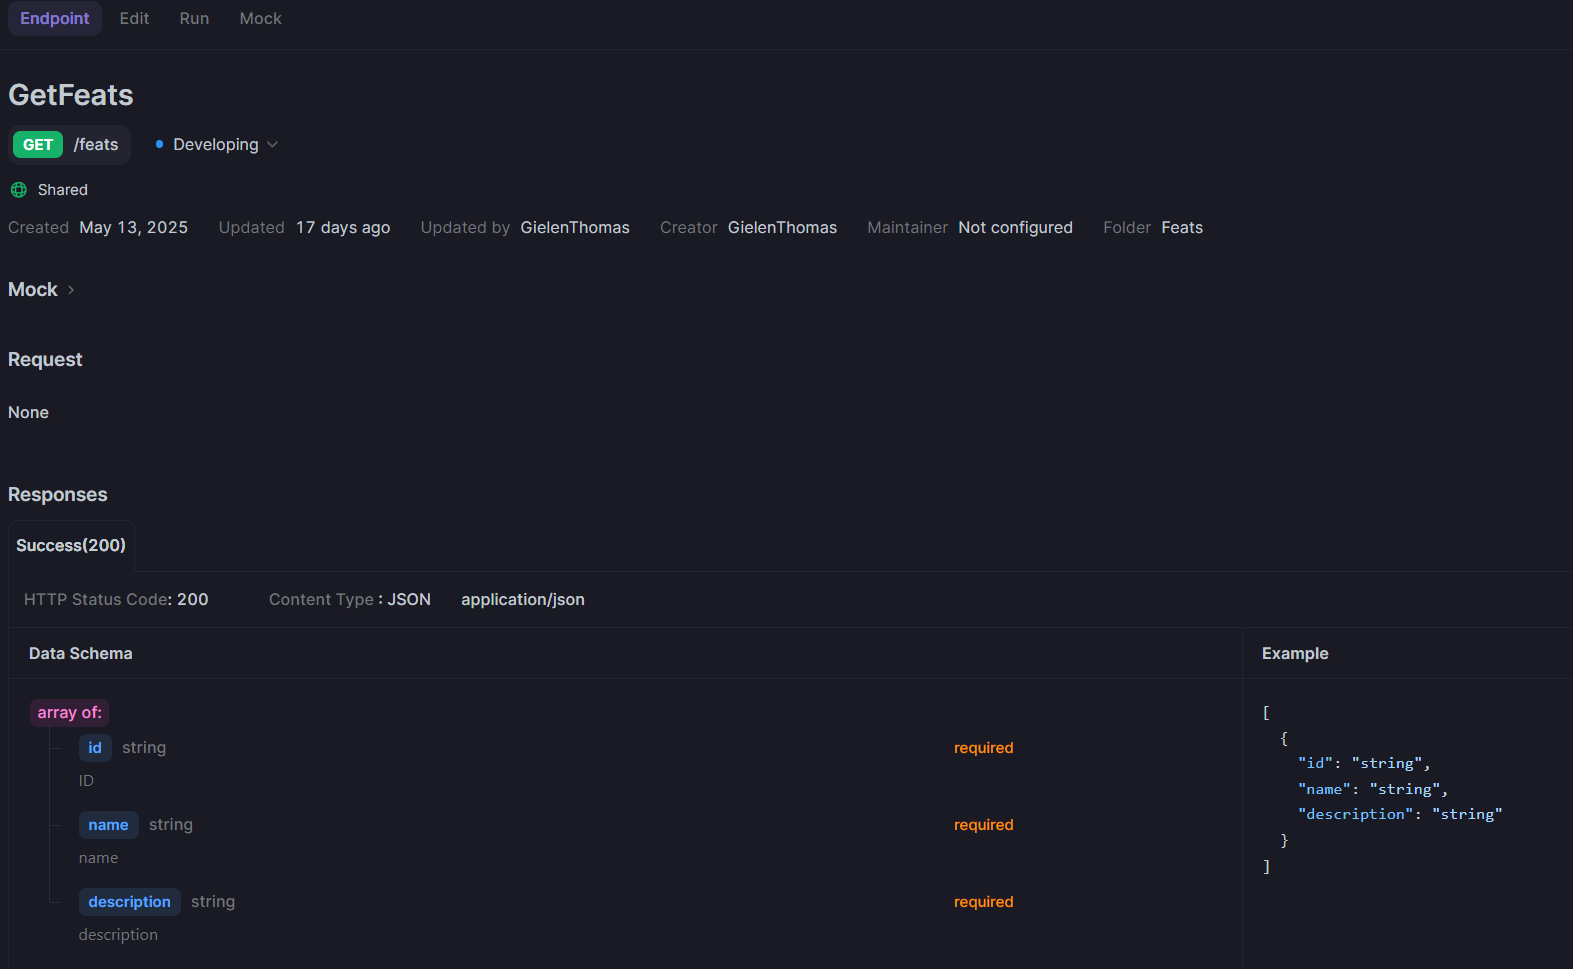
\includegraphics[width=0.8\textwidth]{end-point-voorbeeld.png}
    \caption[Voorbeeld end-point.]{\label{fig:end-point-voorbeeld}Voorbeeld van een endpoint in dogApi}
\end{figure}

\begin{listing}
    \begin{minted}{yaml}
         "/feats": {
             "get": {
                 "summary": "GetFeats",
                 "deprecated": false,
                 "description": "",
                 "tags": [],
                 "parameters": [],
                 "responses": {
                     "200": {
                         "description": "",
                         "content": {
                             "application/json": {
                                 "schema": {
                                     "type": "array",
                                     "items": {
                                         "$ref": "#/components/schemas/FeatResponse"
                                     }
                                 }
                             }
                         },
                         "headers": {}
                     }
                 },
                 "security": []
             },
    \end{minted}
    \caption[openAPIEndPoint]{End-point van de OpenAPI spec}
\end{listing}


\begin{figure}
    \centering
    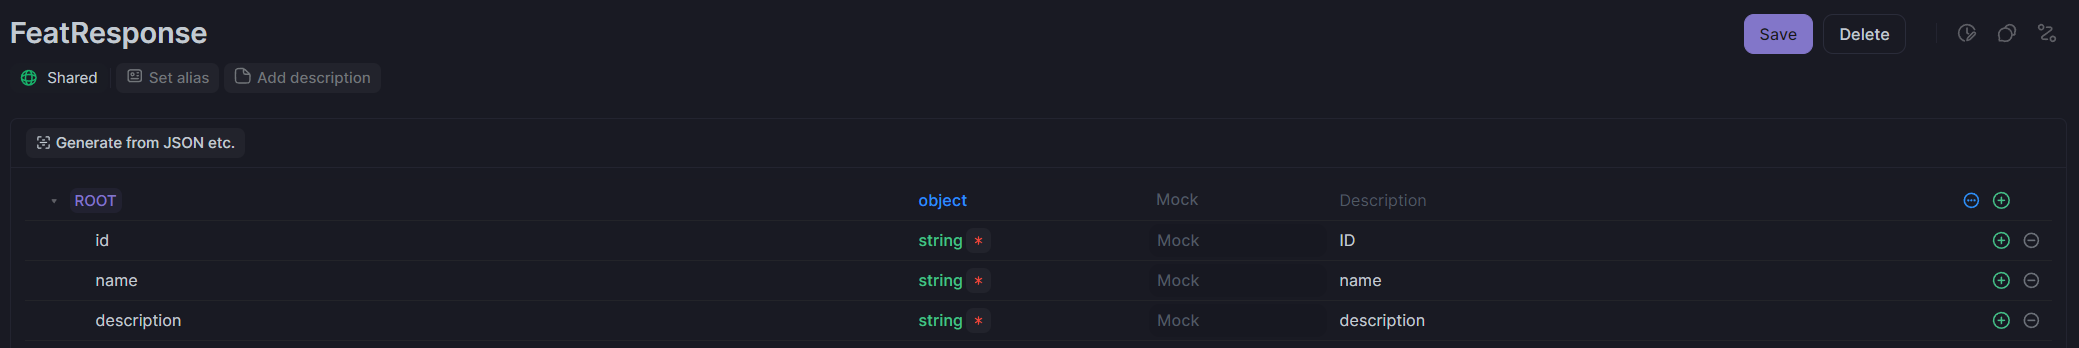
\includegraphics[width=0.8\textwidth]{data-model-voorbeeld.png}
    \caption[Voorbeeld end point.]{\label{fig:data-model-voorbeeld}Voorbeeld van een data model in dogApi}
\end{figure}

\begin{listing}
    \begin{minted}{yaml}
        "FeatResponse": {
            "type": "object",
            "properties": {
                "id": {
                    "type": "string",
                    "description": "ID"
                },
                "name": {
                    "type": "string",
                    "description": "name"
                },
                "description": {
                    "type": "string",
                    "description": "description"
                }
            },
            "required": [
            "name",
            "description",
            "id"
            ]
        },
        \end{minted}
        \caption[openAPIDataModelSpec]{Data model van de OpenApi spec}
    \end{listing}

% Voeg hier je eigen hoofdstukken toe die de ``corpus'' van je graduaatsproef
% vormen. De structuur en titels hangen af van je eigen onderzoek. Je kan bv.
% elke fase in je onderzoek in een apart hoofdstuk bespreken.

%\input{...}
%\input{...}
%...

%%=============================================================================
%% Conclusie
%%=============================================================================

\chapter{Conclusie}%
\label{ch:conclusie}

% TODO: Trek een duidelijke conclusie, in de vorm van een antwoord op de
% onderzoeksvra(a)g(en). Wat was jouw bijdrage aan het onderzoeksdomein en
% hoe biedt dit meerwaarde aan het vakgebied/doelgroep? 
% Reflecteer kritisch over het resultaat. In Engelse teksten wordt deze sectie
% ``Discussion'' genoemd. Had je deze uitkomst verwacht? Zijn er zaken die nog
% niet duidelijk zijn?
% Heeft het onderzoek geleid tot nieuwe vragen die uitnodigen tot verder 
%onderzoek?

Deze graduaatsproef richtte zich op het ontwikkelen van een RESTful API voor het aanmaken en beheren van Dungeons \& Dragons-personages met behulp van het Spring Boot framework en een OpenAPI-gedreven aanpak. Het doel was om een efficiënte, schaalbare en onderhoudbare API te realiseren met moderne technologieën.

Door gebruik te maken van Apidog voor het opstellen van de OpenAPI-specificatie en het automatisch genereren van request- en responseklassen, kon een consistente en gestructureerde API worden gebouwd. Dit verminderde implementatiefouten en zorgde voor een goede afstemming tussen documentatie en code. De implementatie van controllers, services en repositories volgde een duidelijke scheiding van verantwoordelijkheden, wat de onderhoudbaarheid en uitbreidbaarheid bevordert.

MapStruct werd ingezet om DTO’s om te zetten naar domeinmodellen, wat het ontwikkelproces vereenvoudigde en de leesbaarheid verbeterde. Voor data-opslag werd JPA gebruikt en Liquibase zorgde voor gecontroleerd databasebeheer via versiebeheer en migraties, wat de betrouwbaarheid verhoogde.

Het resultaat is een werkende API die voldoet aan de functionele eisen, inclusief gebruikersauthenticatie en ondersteuning voor diverse personageklassen en rassen. De modulaire opbouw en het gebruik van gangbare technologieën maken toekomstige uitbreidingen eenvoudiger.

Er zijn echter ook beperkingen vastgesteld. Zo ontbreken uitgebreide performancetests, wat nodig is om de schaalbaarheid te garanderen.

De resultaten kwamen grotendeels overeen met de verwachtingen, maar er ontstonden ook nieuwe vragen, zoals hoe de API beter kan omgaan met hoge belasting en hoe integratie met andere Dungeons \& Dragons-tools kan plaatsvinden.

Kortom, deze graduaatsproef leverde een concrete en toepasbare oplossing die bijdraagt aan het vakgebied door een praktische toepassing van moderne Java-technologieën en een OpenAPI-gedreven ontwikkelproces. Voor toekomstig werk is er ruimte voor een front-end voor deze back-end te ontwikkelen en veredere uitbrijdingen voor de back-en te schrijven zoals bevoorbeeld het moegelijk te maken om de characters te laten levelen.



%---------- Bijlagen -----------------------------------------------------------

\appendix

\chapter{Onderzoeksvoorstel}

Het onderwerp van deze graduaatsproef is gebaseerd op een onderzoeksvoorstel dat vooraf werd beoordeeld door de promotor. Dat voorstel is opgenomen in deze bijlage.

%% TODO: 
%\section*{Samenvatting}

% Kopieer en plak hier de samenvatting (abstract) van je onderzoeksvoorstel.

% Verwijzing naar het bestand met de inhoud van het onderzoeksvoorstel
%\input{../voorstel/voorstel-inhoud}

%%---------- Andere bijlagen --------------------------------------------------
% TODO: Voeg hier eventuele andere bijlagen toe. Bv. als je deze BP voor de
% tweede keer indient, een overzicht van de verbeteringen t.o.v. het origineel.
%\input{...}

%%---------- Backmatter, referentielijst ---------------------------------------

\backmatter{}

\setlength\bibitemsep{2pt} %% Add Some space between the bibliograpy entries
\printbibliography[heading=bibintoc]

\end{document}
